%!TEX root=thesis.tex This is the draft literature review.

%!TEX ROOT = thesis.tex


\chapter{Background Study} 
\label{section:litreview}

In this chapter, related theoretical background concepts are first introduced.
Then, the related works in literature are discussed at length in two main sub-sections:
\begin{enumerate}
 \item Existing methodology and techniques used for semantic extraction.
 \item Recent methodology and techniques used for semantic retrieval.
\end{enumerate}



\section{Related Theoretical Background Concepts}
\label{subsec:relatedConcepts}

Before diving deeper into the details of the proposed framework,
the fundamental background towards selected theoretical concepts that are frequently encountered in this work is first discussed. As this thesis covers a broad spectrum of
different concepts, a general treatment of these concepts would provide
some degree of clarity towards the topic at hand. This section briefly describes
some fundamentals of the following concepts: i) Quantisation, ii) Distance
Measure, iii) Human Visual System, \& iv) Colour Model and Colour Terms.


\vspace{1em}
\subsection{Quantisation}

The use of quantisation in the mathematical and digital signal processing fields
is not a new concept; it is commonly applied in various use cases where analogue signals are to be discretised. Digital
signal processors are limited by natural boundaries such as hardware
limitations, and are only able to compute and perform arithmetic operations
within a limited range \cite{spors_2018}. Technically speaking, quantisation refers to the
process of mapping and projecting a set of infinitely large values that is
continuous or analogue in nature into a set of discrete and finite values.

\begin{figure}[hbt!]
 \centering
 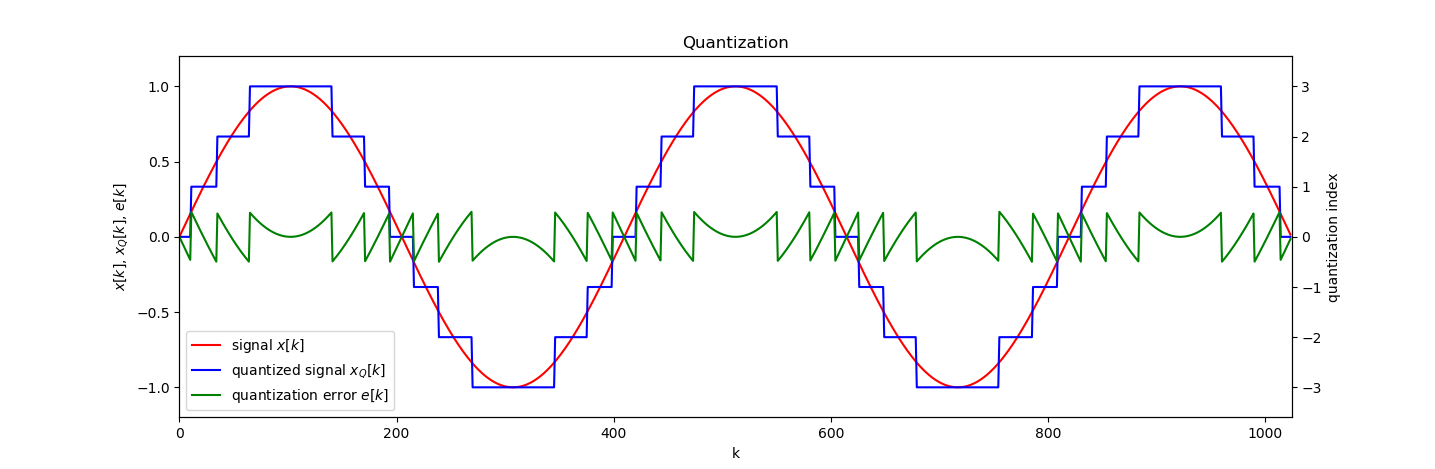
\includegraphics[width=\textwidth]{image/general/quantization.png}
 \caption{Illustration of the Quantisation Process}
 \label{fig:quantize}
\end{figure}

The use of quantisation enables reduction in memory usage (\emph{i.e.} compression in terms of lesser bit representation) and
reduction of computational cost which leads to faster processing speed.
However, since the quantisation process is a \emph{many-to-few} mapping
operation, the operation is considered irreversible without prior knowledge of
the loss. Hence, the output discrete signal can closely resemble the continuous input signal if a large number of quantisation levels are used.

In order to expound on the quantisation process, a mathematical model of this
process is given as:
\begin{equation}
 \centering
 \label{eq:quantization}
 x_Q[k] = g(\mspace{3mu}\lfloor \mspace{3mu}f(x[k]) \mspace{3mu}\rfloor\mspace{3mu})
\end{equation}
\vspace{-3em}
\begin{equation}
 \centering
 \label{eq:quantizationerror}
 e[k] = x_Q[k] - x[k]
\end{equation}
where a continuous signal $x[k]$ whose
corresponding quantised signal, $x_Q[k]$, is desired (see Equation \ref{eq:quantization}). The
functions $f (\mspace{3mu} \cdot \mspace{3mu})$ \& $g (\mspace{3mu} \cdot\mspace{3mu})$
can be regarded as a real-value mapping function while $\lfloor \mspace{3mu} \cdot
\mspace{3mu} \rfloor$ represents a rounding function. The function $
f(\mspace{3mu} \cdot \mspace{3mu})$ is used to
convert real-world values into a discrete-level signal, while function
$g (\mspace{3mu} \cdot\mspace{3mu})$ maps the digital signal into a
quantised signal of a predetermined level. As mentioned, this process is considered irreversible without
prior knowledge of the loss. In this case, the quantisation error, $e[k]$, can be
computed as Equation \ref{eq:quantizationerror}. Figure \ref{fig:quantize}
illustrates the quantisation process where the red signal ($x[k]$) represents
the real-world continuous signal, the blue signal ($x_Q[k]$) refers to the
quantised signal while the green signal ($e[k]$) represents the error due to
quantisation process.

To further leverage on this concept, the quantisation technique
can be extended into three-dimensional (3D) space, as it is done in this work. As video data is represented in 3D space (\emph{i.e.} X-axis, Y-axis, and T-axis for time), the quantisation process is used to map continuous video data into a set of discrete
and finite values. These discrete values are then used to further ease the
calculation and manipulation of data. Likewise, as colours can also be
represented using 3D space (\emph{i.e.} most colour spaces consists of a triplet of channels), this concept can be adapted and applied to quantize the colour space into several dominant colours accompanied
with the assignment of colour terms (See Section \ref{section:colourterm}).



\vspace{1em}
\subsection{Distance Measure}
\label{section:distancemeasures}

The use of distance measure is another recurring key concept in the proposed
methods. Distance measures are simply a numerical measurement between
two or more points or objects. According to \cite{mccune2002distance},
distance measures are flexible and can be measured as either a distance (or a dissimilarity)
or a similarity, both respectively being concepts inverse to each other. As such, most distance measures can be readily converted into
similarities and vice versa. 
%They can also be categorised as metric semmetric or nonmetric.
As distance measures are commonly used in the mathematics and
computer science fields, there are numerous metrics suggested by different
authors which are applicable in different scenarios. It is also
vital to obtain an acceptable range of values for each distance measure, as according to its application of use.

\begin{figure}[hbt!]
 \centering
 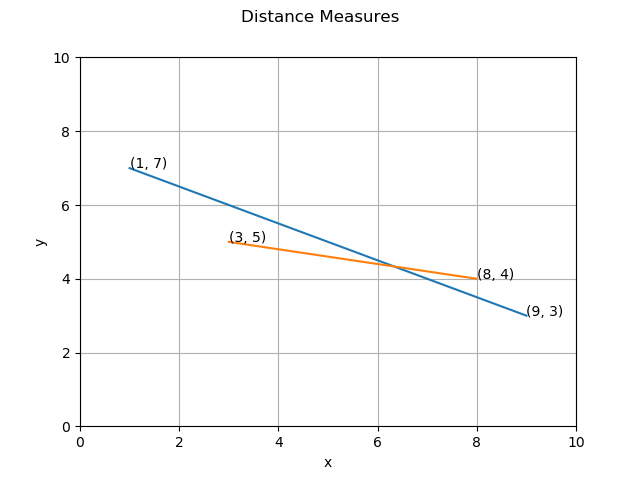
\includegraphics[width=.7\textwidth]{image/general/distance.png}
 \caption{Example of Distance Measure.}
 \label{fig:distanceMeasure}
\end{figure}

To further elaborate on the concept of distance measure, a simple
example of how distance metrics can be applied in this research is
illustrated in Figure \ref{fig:distanceMeasure} with two plotted lines.
In our research problem, these lines can be regarded as vehicle
trajectories captured over time, visually flatten unto a 2D plot. Using such spatio-temporal data and assuming time is taken at a fixed interval, the distance between two trajectories can be measured to signify
the dissimilarity between them. This distance measure, or similarity score (if inverted), can also be used to
identify trajectories with high resemblance. For example, the distance between these two lines can be measured using $D_{Euclidean} = \sum^n\sqrt{{(A_n[x] - B_n[x])}^{2} +{(A_n[y] - B_n[y])}^{2}}$ which results to 2.828427 units. As Euclidean Distance requires the length of both lines or vectors to be equal, a common approach is to apply the zero-padding technique to extend the shorter vector.

\begin{figure}[hbt!]
 \centering
 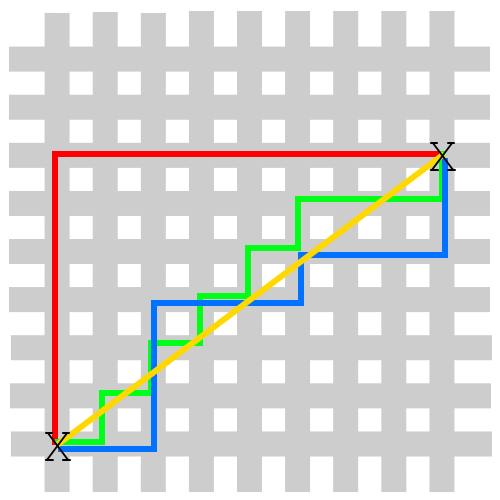
\includegraphics[width=.5\textwidth]{image/lit/manhattan.png}
 \caption[Comparison between Manhattan Distance vs. Euclidean Distance]{Comparison between Manhattan Distance vs. Euclidean Distance. The yellow diagonal line connecting both \emph{X} represents the Euclidean Distance while the other lines represents the various solution obtainable using Manhattan Distance.}
 \label{fig:manhattan}
\end{figure}

However, as different distance measure metrics are suitable for different
scenarios, a good distance measure is vital for comparing a significantly
extensive set of vehicle trajectories from a car park scene for the purpose of video shot retrieval. This concept of distance measure can be further extended to other
multi-dimensional spaces such as the colour space, where the similarity between
two or more colours can be similarly measured using different distance metrics. 
%to evaluate the performance of each metric. 
Table \ref{table:distance} lists several
distance measures which are commonly used along with their respective pros and cons while Figure \ref{fig:manhattan} contrasts the two popular distance metrics -- the Euclidean ($\ell 2$-norm) distance and the Manhattan ($\ell 1$-norm) distance. 
With the assumption that each block has a equal distance of 1. Using Manhattan Distance, regardless of the path taken, the distance for the red, green and  blue lines has the length of $14$. These 3 paths, while different, still takes on the shortest distance from one end to the other. However, when computing using Euclidean Distance, the distance is measured to be $\sqrt{8^2+6^2} = 10$. Euclidean Distance only produces $1$ unique solution while Manhattan Distance may produce more than one solution.
Further comparison between several distance measures is
also discussed in Chapter 4 to understand and validate the chosen distance
measure for each of the proposed methods.

% CLARENCE: Add more distance measure, especially those that u included for
% chapter 5

\begin{table}[!ht]
\caption{List of Several Popular Distance Measures %and Their Pros and Cons
}
\resizebox{
\textwidth}{!}{
\begin{tabular}{|l|l|l|} \hline
\textbf{Distance Measure} & \textbf{Pros} & \textbf{Cons} \\ \hline
Euclidean Distance & \begin{tabular}[c]{@{}l@{}}Simple, Fast,\\ Commonly used,\\ Able to
work on n-Dimension data\end{tabular} & \begin{tabular}[c]{@{}l@{}}Vector
order dependent,\\ Requires same length vectors\end{tabular} \\ \hline
Manhattan Distance & \begin{tabular}[c]{@{}l@{}}Reflection invariant,\\
Translation invariant,\\ Produces same result,\\ Able to work on n-Dimension
data\end{tabular} & \begin{tabular}[c]{@{}l@{}}Requires same length
vectors,\\ Does not have a unique solution\end{tabular} \\ \hline
Chamfer Distance & \begin{tabular}[c]{@{}l@{}}Able to work with \\ vectors of
different length,\\ Vector order invariant, \\ Minimises the difference \\
between vectors,\\ Able to work on n-Dimension data\end{tabular} &
\begin{tabular}[c]{@{}l@{}}Higher computational cost,\\ Alternative matches
may \\ receive equal distance\end{tabular} \\ \hline
Hamming Distance & \begin{tabular}[c]{@{}l@{}}Ensure similarity between vectors,\\ Able to work
on n-Dimension data\end{tabular} & \begin{tabular}[c]{@{}l@{}}Vector order
dependent,\\ Requires same length vectors\end{tabular} \\ \hline
\end{tabular}}
\label{table:distance}
\end{table}
 

\vspace{1em}
\subsection{Human Visual System}
An interesting excerpt by \citeA{albers2006interaction} states that ``In order to use colour effectively it is necessary to recognise that colour deceives continually. To this end, the beginning is not a study of colour systems.
First, it should be learned that one and the same colour evokes innumerable readings. Instead of mechanically applying or merely implying laws and rules of colour harmony, distinct colour effects are produced-through recognition of the interaction of colour-by making, for instance, two very different colours look alike, or nearly alike''. Hence, the human visual system is first explored to understand how to use colours effectively.

\label{section:eyes}
The human eyes are visual biological organs responsible of receiving and
processing visual stimuli. Figure \ref{fig:eyes} shows a rough anatomy of
the human eye. Within the eye, rods and cones are light-sensitive cells
found on the retina which are in charge of vision. Both of these cells play
a different role; rod cells are not able to perceive colour information, as such, they are known to be responsible for sensing changes in light intensities.
On the other hand, cones cells are responsible for the reception of colour
information. As the human retina contains approximately 120 million rods and
6 million cones, the human eyes are more sensitive toward lighting conditions.
The sheer number of rods also enables humans to see in low-light achromatic
vision.


\begin{figure}[hbt!]\centering
 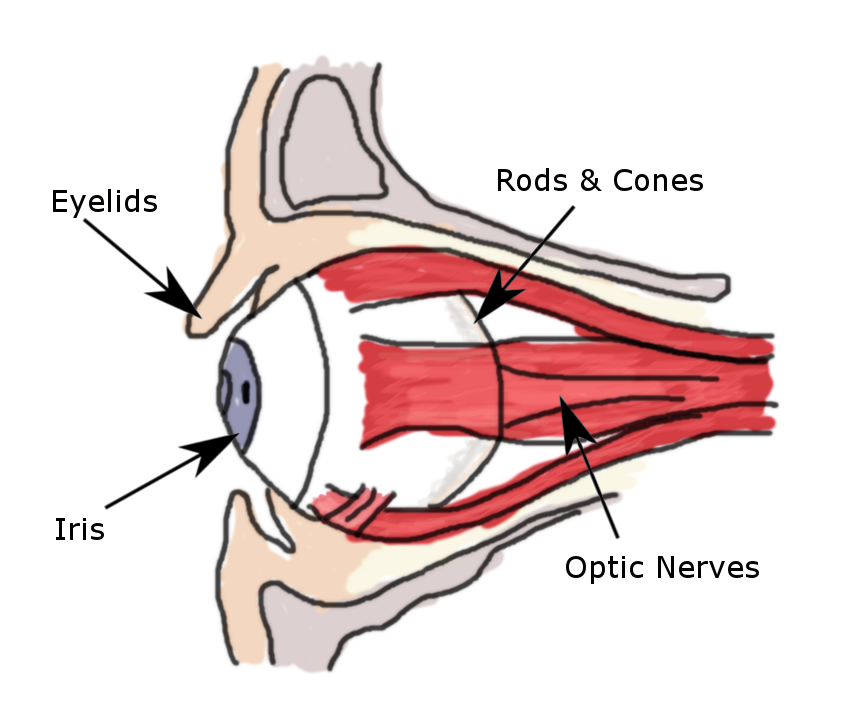
\includegraphics[width=.5\textwidth]{image/lit/rodsandconscolored.png}
 \caption[Human Eye Anatomy]{Human Eye Anatomy. Rods and cones cells are
 responsible over human vision. %When these cells on the retina are stimulated,  signals are sent to the brain via the optic nerves. The brain would then processes these signals to provide vision for humans.
 }
 \label{fig:eyes}
\end{figure}

Anatomically, there are three types of cones in the human retina, each of which
are responsible over the receptiveness of colours in a particular set of
wavelengths. These wavelengths can be classified into three main categories:
Short wavelength light, Medium wavelength light and Long wavelength light, as shown in Figure \ref{fig:visibleSpectrum} \cite{eyespectrum}. Overall, colours are perceived from the combination of stimuli to these rods, cones cells and responses from
brain. When stimulated, these cells trigger electrical signals to the optic nerve
fibres which then communicates it to the brain. However, as the number of cone cells
in the retina varies for each person, the colour perception of every person may differ from one another.


\begin{figure}[hbt!]
 \centering
 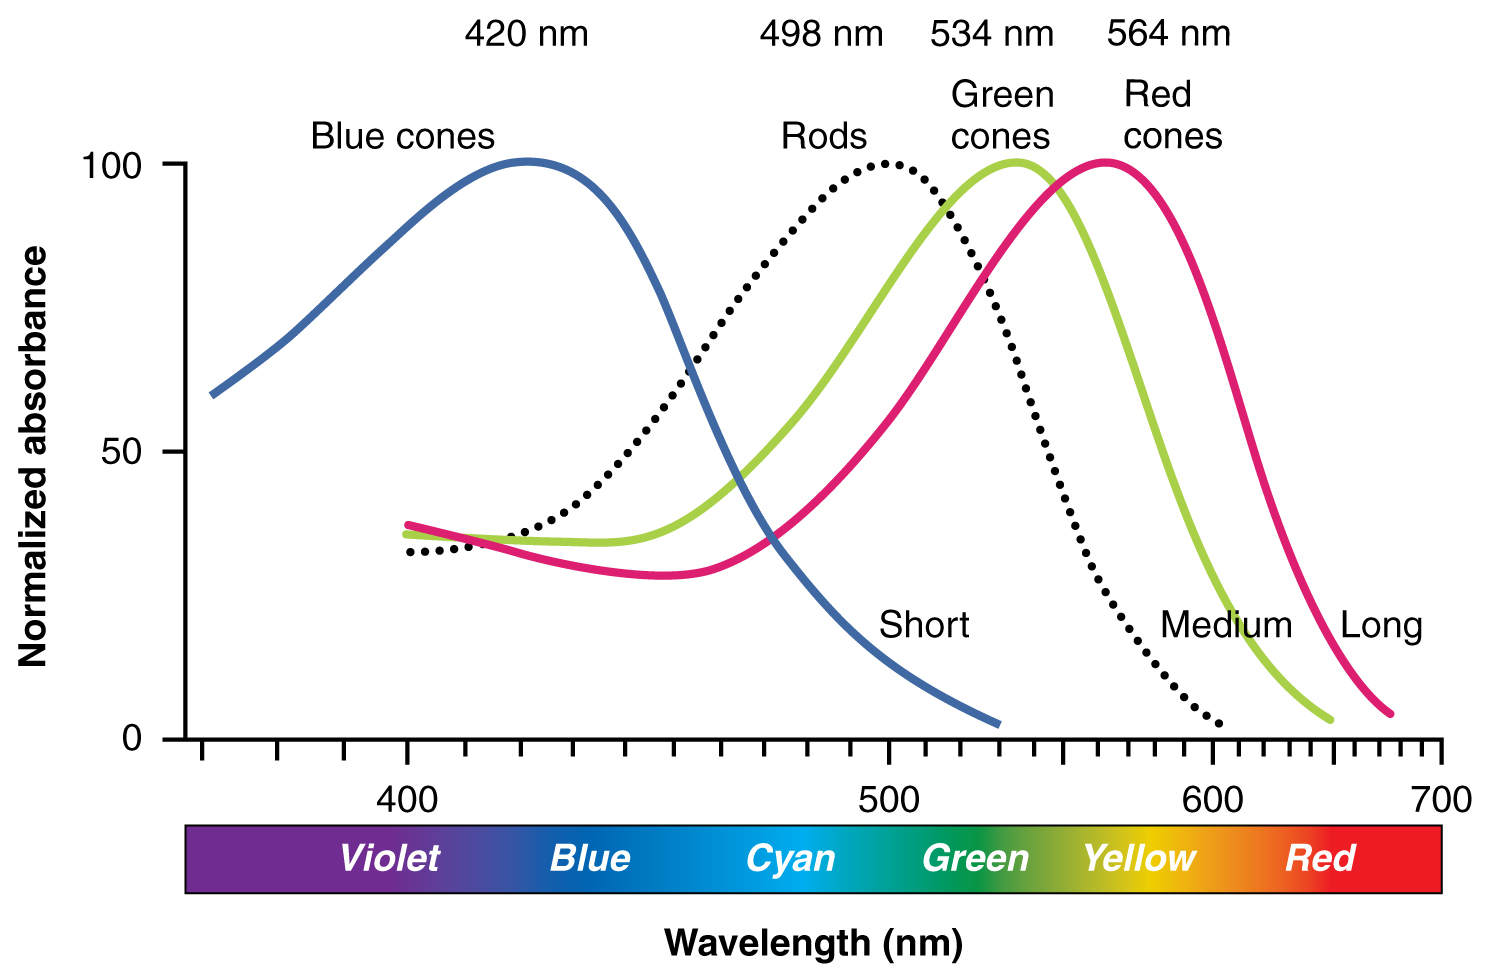
\includegraphics[width=.7\textwidth]{image/lit/ColorSensitivity.jpg}
 \caption[Normalised Human Photo-Receptor Absorbency Rate for Different
 Wavelength Lights]{Normalised Human Photo-Receptor (Cones \& Rods) Absorbency
 Rate for Different Wavelengths of Light. %'Blue' Cones, Approximately 420-440 nm, are Short Wavelengths Light; 'Green' Cones, Approximately 534-545 nm, are Medium Wavelengths Light; and, 'Red' Cones, Approximately 564-580 nm, are Long Wavelength Lights. 
 }
\label{fig:visibleSpectrum}
\end{figure}


\vspace{1em}
\subsection{Colour Model, System and Terms}
\label{section:colourterm}

In order to represent colours in modern computers, colour models were designed
to such that colours can be digitally represented using a series of number
tuples~\cite{travis1991effective}. In essence, it is a quantisation process of converting
a series of real-world continuous signals (colour wavelengths) into a set of
finite tuples of numbers within a colour model. This quantisation process enables 
%With the ability to quantize
%these wavelengths into sets of finite tuples, the 
colour information to be stored digitally for further processing.


\vspace{1em}
\subsubsection{RGB Colour Model}
In the previous section, the humans visual system is briefly described to contain 
%was explored. From there, we learn that the 
cones cells in the retina that are strongly receptive towards visual stimuli containing 'Red', 'Green' and 'Blue' wavelengths.
The RGB colour model is designed based on the theory behind human perception
of three distinct colour wavelengths in mind ~\cite{travis1991effective, young1802ii}. This colour model is commonly used to represent and display images in digital devices and systems.

% comment: No other colour spaces are described here. So it is just RGB
%As an example, the 
The RGB colour space is an additive colour model, where each of its
components (R, G, B) are added together to produce the final colour. Typically, each of these components are represented using 8 bits, resulting in a total of 256 possible values
for each component with a combined total of $256 \times 256 \times 256 = \sim 16M$ colours overall. As this is an additive model, 'Black' colour is
represented using $(0, 0, 0)$ (no colours present), while 'White' is represented by $(255, 255, 255)$ (colours fully present). 
% Figure~\ref{fig:rgb} represents this colour model.

% \begin{figure}[hbt!]
%  \centering
%  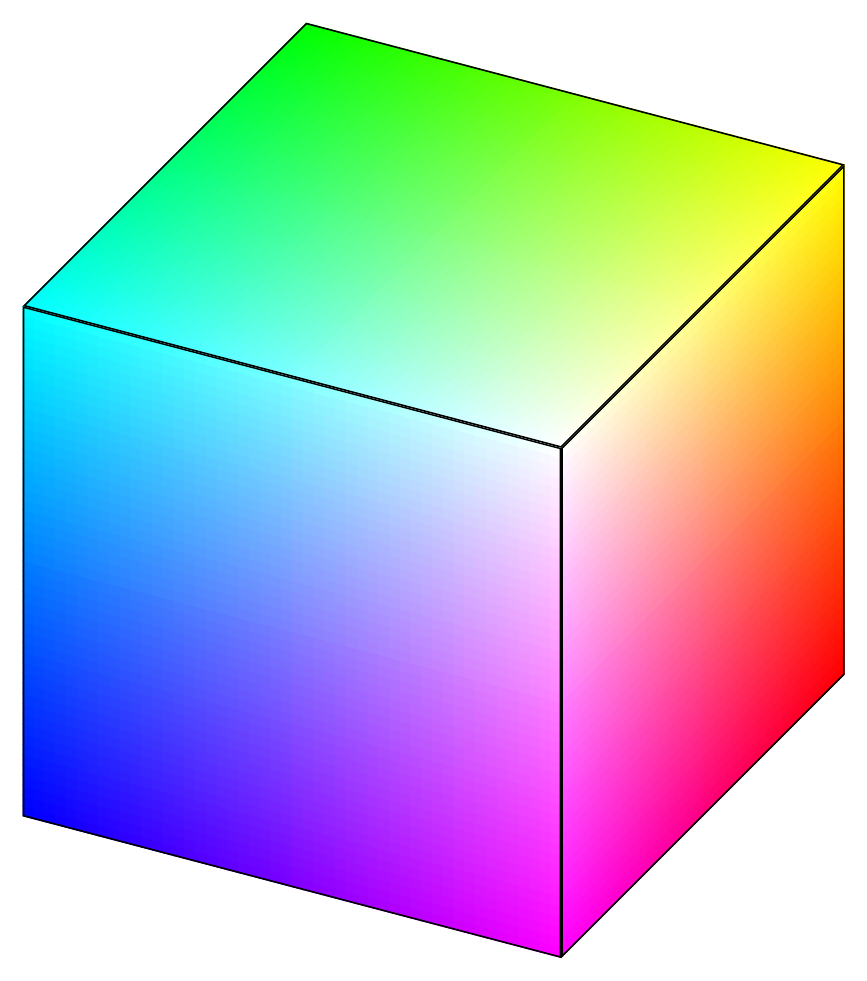
\includegraphics[width=.4\textwidth]{image/lit/rgbcolor.jpg}
%  \caption{RGB Colour Model}
% \label{fig:rgb}
% \end{figure}


\vspace{1em}
\subsubsection{Munsell Colour System}
\label{section:munsellcs}
Colour terms - such as ``Red'', ``Green'' or ``Blue'', are commonly derived from
the Munsell colour system which was created in the early 20th century by
Professor Albert H. Munsell. The Munsell colour System was designed to organise colours similar to how the human eye sees - which is, by
organising colours according to their hues, followed by the chromatic range
and the brightness values in a perceptually uniform manner. In the words of
Munsell, ``It may sound strange to say that colour has three dimensions, but it
is easily proved by the fact that each of them can be measured separately.''
% note: added further elaboration on why other colour spaces (HSV, LAB) are not used
The classic RGB colour space is not known to possess perceptually uniform components as the Euclidean distance between its colour components does not correspond to the colour differences perceived by humans~\cite{paschos2001perceptually}. Although there exists perceptually uniform colour spaces such as L*a*b*, as well as approximately-uniform colour spaces such as HSV, these colour spaces are not intuitively descriptive for mapping to specific color terms.

Figure \ref{fig:munsell} depicts the Munsell Colour System. In the horizontally lying circle on the Munsell Colour System, the segments can be divided into 5 principle hues which are Red, Yellow, Green, Blue, and Purple. This setup
allows another 5 intermediate hues in between each principle hues, \emph{e.g.} Green-Blue hue, Purple-Red hue. Figure \ref{fig:munsell}(b) illustrates the property of the chroma and value scale available on the Munsell colour system, for
instance, a hue at 2.5 Yellow-Red (YR) has a maximum chroma value which differs
along the value axis.

\begin{figure}[!htb]
 \centering
 \resizebox{\textwidth}{!}{
 \begin{tabular}{cc}
 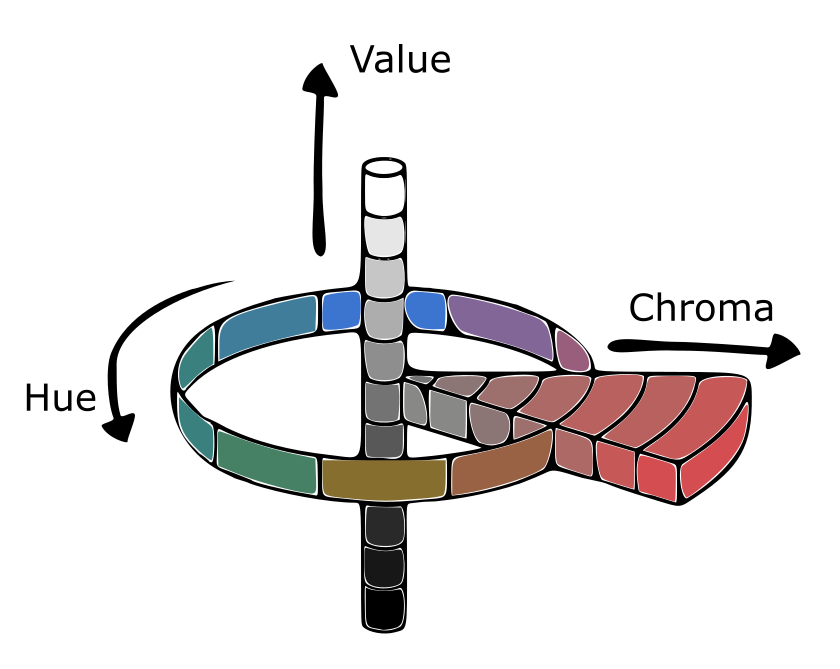
\includegraphics[width=0.4\linewidth]{image/general/munsell.png} &
 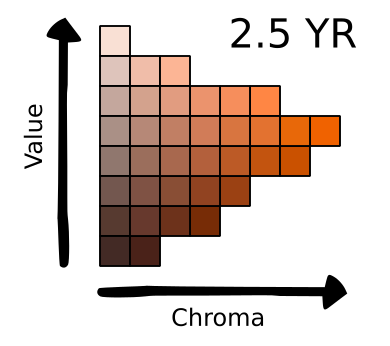
\includegraphics[width=0.4\linewidth]{image/general/25YR.png}\\ (a) Munsell
 colour System & (b) Hue at 2.5YR with various Chroma and Value\\
 \end{tabular}}
\caption{Munsell Colour System}
\label{fig:munsell}
\end{figure}


\vspace{1em}
\subsubsection{Colour Terms}

While the idea of colours seems to be a relatively simple idea for humans,
machines do not understand the concept of colours. Modern
computers generally represent colour values using the Red-Green-Blue (RGB)
values for most applications. Despite its frequent usage, it is difficult for
humans to visualise a particular colour when presented with three RGB values as
these values do not directly translate intuitively to a particular
colour. Along with that, it is also very difficult to visualise the difference or the `distance'
between two colours solely using the RGB values only; hence, these values are not perceptually meaningful.

Table \ref{table:allcolourterms} lists several popular web colour dictionaries
along with the number of colour terms and the publishing year. One
notable property of these colour terms is the use of compound terms such as
`baby blue', `dark red', `light purple' and `very deep brown', all of which indicates a fine disambiguation between shades of the same hue.
Also, in certain colour dictionaries, colour terms are somewhat duplicated for several tuple of values. An interesting note by \citeA{de1971color} puts the difficult plainly: ``The explanation of the nature and essence of colour gives such difficulty that the opinions of nearly all physicians are divided''. Given the variety of colour dictionaries and the broad range of different colour terms, this work also indirectly investigates into the number of colour terms that should be allocated to describe the wide range of vehicle colours.

\begin{table}[hbt!]
 \caption[Web Colour Dictionary and the Corresponding Number of Colour Terms]
 {Various Common Web Colour Dictionaries. Compiled from Various Source ~\cite{jaffer_2017, raveling, crayolacolor} %and the Corresponding Number of Colour Terms
 }
 \centering
 \begin{tabular}{|c|c|c|} \hline
 \multicolumn{1}{|c|}{\textbf{Web Colour Dictionary}} &
 \multicolumn{1}{c|}{\textbf{Number of Colour Terms}} &
 \multicolumn{1}{c|}{\textbf{Publishing Year}} \\ \hline x11 (R3)
 & 631                         & 1988
 \\ \hline HTML                        & 140
 & Current              \\ \hline CSS
 & 148                         & Current
 \\ \hline Crayola                       & 250
 & Current              \\ \hline xkcd
 & 954                         & 2010
 \\ \hline
 \end{tabular}
\label{table:allcolourterms}
\end{table}
%https://people.csail.mit.edu/jaffer/colour/Dictionaries x11 colours:
 %https://groups.google.com/forum/?fromgroups=#!topic/comp.windows.x/AYPozZhQxok
 %https://www.crayola.com/explore-colours.aspx
 %http://markkness.net/colourpy/colourPy.html

Historically speaking, in a classic study on worldwide colour naming, \citeA{berlinandkay} commented
that the naming of colours terms may differ due to different cultures. Based on their findings, native English language speakers generally used eleven basic colour terms. These terms had to have three common properties which are: 1) Highly used, 2) Monolexemic -- meaning a single (mono) word, and not compounded colour terms such as `baby blue', and 3) agreed upon by native speakers of the language. With those definitions, the common colour terms proposed for the English language are black, white, gray, brown, red, orange, yellow, purple, green, blue, and pink. These 11 common colour terms were also adopted by
several other authors (\citeA{van2009learning}, \citeA{zaslavsky2018efficient},
and \citeA{yu2018beyond}) in their work to understand how these colour
terms can be used for real-world image applications.
However, \citeA{yu2018beyond} also remarked that most existing work on colour names focuses only on the 11 aforementioned basic colour terms of the English language.
However, this could potentially either limit or incorrectly represent the actual range of colours in an outdoor car park scenario; this warrants further investigation in this research. %the discriminative power of these representations.


\section{Related Works in Literature}
\label{section:relatedworks}

The advancement of computer vision technologies enabled the development and
integration of various solutions to tackle challenges in Intelligent
Transportation Systems (ITS). As ITS is a large topic by itself, there has been a substantial increase of research done on the various sub-domains.
To avoid re-inventing the wheel, existing frameworks are thoroughly reviewed in this section to find potential adoption if relevant and to uncover potential gaps in literature. Recent survey done by \citeA{tian2017hierarchical} and
\citeA{chandran2017review} provide a general overview of the state of related works. The authors summarised the challenges that are
often found in an ITS setting that is implemented on a one-camera setup:
\begin{enumerate}[label=(\alph*)]
 \item \textbf{Camera placement} affects the overall performance.
 \item The \textbf{lighting condition} varies throughout the day. Supplemental lighting equipment can be used during the night, however, the visual range will be limited.
  \item Vehicles are often \textbf{occluded} in an ITS setting; often by pedestrians, bicycles, trees, and even buildings.
 \item \textbf{Vehicle pose} varies when turning or changing lanes.
 \item Vehicles comes in a \textbf{variety of shapes, sizes, and colour.}
 \item \textbf{Vehicles' size changes} as they pass through the camera's field of view. This variation in visual information affects the robustness of some detection models.
\end{enumerate}
Along with that, \citeA{tian2017hierarchical} presented an overview of the
general frameworks for ITSs with the aim of vehicle attribute extraction and
behaviour understanding, as shown in Figure \ref{fig:ITSoverview} where `Layer 1' describes the process of obtaining data via vision sensors, `Layer 2' -- Attribute
Extraction from data; this includes motion, trajectories, colours, shapes
and etc. `Layer 3' -- Analysis on vehicle behaviours from the extracted
attributes to decide traffic status. Lastly, `Layer 4' describes how information from `Layer 3' can be utilises to optimise various ITS services. 
According to
\citeA{liu2016deep}, in a real-world scenario, appearance features such as
colours, shapes, and types are very effective at filtering out dissimilar
vehicles. In addition, they are efficient to be extracted and searched in a 
large-scale dataset. 

As mentioned in Section \ref{subsec:scope}, the scope of work in this thesis assumes that the
bounding box of each vehicle have been obtained prior to the semantic
extraction task. As such, related literature regarding the detection and tracking of
vehicles is omitted from discussion. Instead, the rest of this section covers two main tasks: Objects Semantic Extraction and Object Semantic Retrieval.


\begin{figure}[hbt!]\centering
 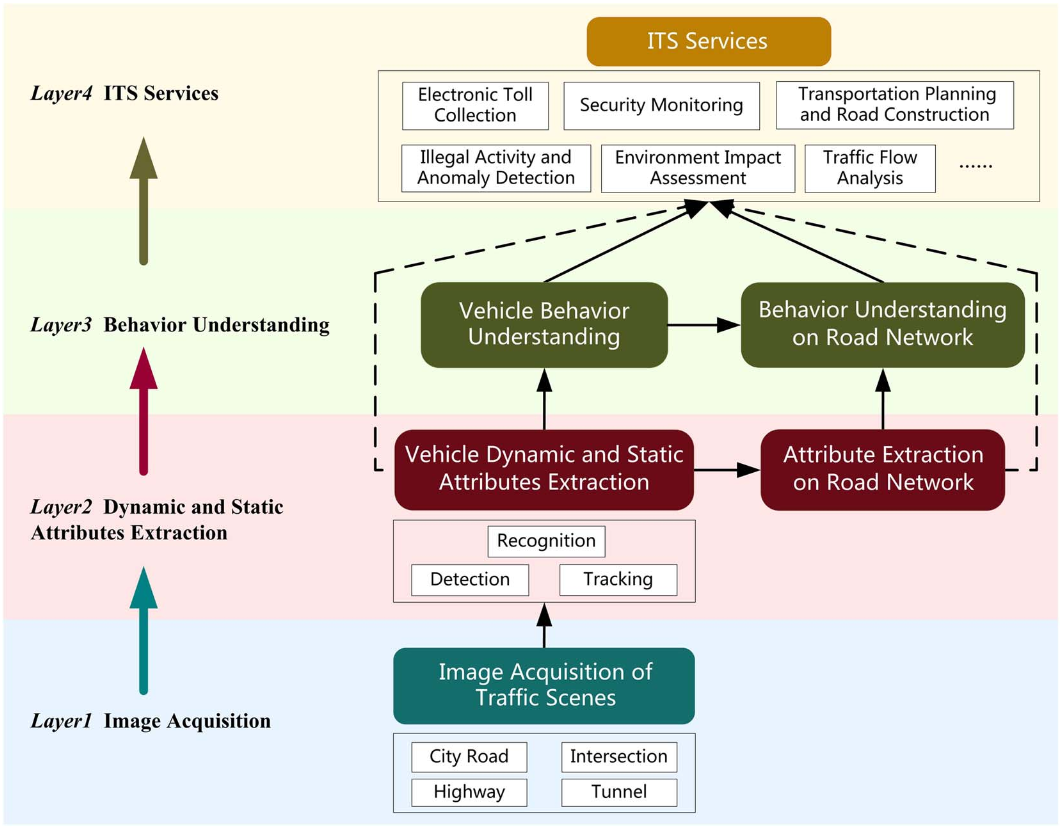
\includegraphics[width=1\textwidth]{image/lit/ITS.png}
 \caption[Overview of the General Frameworks for ITSs]{Overview of the General Frameworks for ITSs 
 %(From Bottom) 
 Figure reproduced
 from~\citeA{tian2017hierarchical}}
 \label{fig:ITSoverview}
\end{figure}


\vspace{1em}
\subsection{Object Semantics Extraction}

Three relevant sub-topics are presented in this section: Vehicle colour extraction, colour to colour term mapping, and vehicle motion extraction and representation.

\vspace{1em}
\subsubsection{Vehicle Colour Extraction}
The extraction of vehicle colours is essential for a wide variety of
applications in ITS, such as crime prevention, vehicle re-identification and video shot retrieval purposes.
According to \citeA{zhang2017vehicle}, colour is one of the
most stable attributes of vehicles and is often used as a valuable cue in some
important applications. Works by \citeA{hsieh2015vehicle}, \citeA{chen2014vehicle} and
\citeA{zhang2017vehicle} noted that in a surveillance scenario, the varying
illumination, coupled with complex environment factors (weather, noise) as well as the camera viewpoint in an outdoor scene affects the classification of colours drastically. 


Various vehicle colour extraction methods has been proposed in the recent
years, and they can be broadly divided into two main categories:
i) hand-crafted features, and ii) machine-learned features. 

\begin{figure}[hbt!]
 \centering
 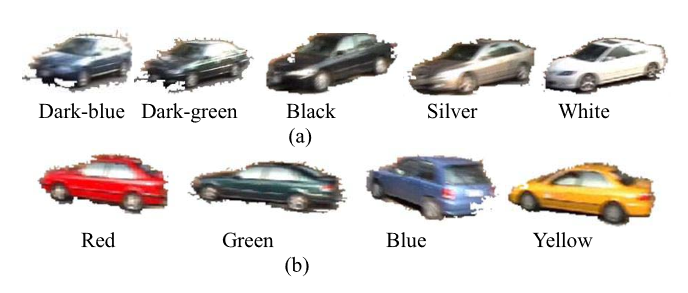
\includegraphics[width=.8\textwidth]{image/lit/carscolors.png}
 \caption[Colour Appearance Categories of Vehicle Used for Colour
 Classification]{Vehicles Classified as (a) Achromatic, and 
 (b) Chromatic. Reproduced from \citeA{hsieh2015vehicle}.}
\label{fig:sevenclasses}
\end{figure}

\begin{figure}[!htb]
 \centering \resizebox{\textwidth}{!}{ \begin{tabular}{ccc}
 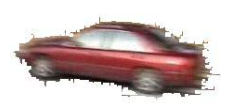
\includegraphics[width=0.4\linewidth]{image/lit/windowremove1.png} &
 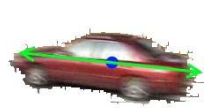
\includegraphics[width=0.4\linewidth]{image/lit/windowremove2.png} &
 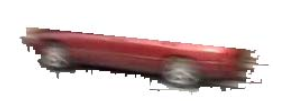
\includegraphics[width=0.4\linewidth]{image/lit/windowremove3.png} \\ (a)
Input Vehicle & (b) Proposed Cutting Line for Window Removal & (c) Result of
Window Removal\\ \end{tabular} }
 \caption[Window Removal Task. From left: Input
Vehicle, Proposed Cutting Line, Results of Window Removal]{Window Removal Task.
From left: Input Vehicle, Proposed Cutting Line, Results of Window Removal.
Image reproduced from \citeA{hsieh2015vehicle}
 \label{fig:windowremoval}}
\end{figure}

\begin{figure}[!htb]
 \centering \resizebox{\textwidth}{!}{ \begin{tabular}{cccc}
 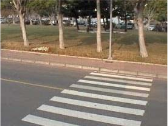
\includegraphics[width=0.3\linewidth]{image/lit/cc1.png} &
 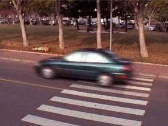
\includegraphics[width=0.3\linewidth]{image/lit/cc2.png} &
 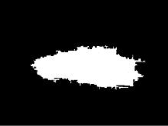
\includegraphics[width=0.3\linewidth]{image/lit/cc4.png} &
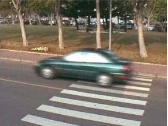
\includegraphics[width=0.3\linewidth]{image/lit/cc3.png} \\ (a) Reference Image
& (b) Colour Distortion & (c) Background of (b) & (d) Result of Colour
Correction\\
 \end{tabular} }
 \caption[Colour Correction. From left: Reference Image, Image with Colour
 Distortion, Background of (b), Results of Colour Correction]{Colour
 Correction. From left: Reference Image, Image with Colour Distortion,
 Background of (b), Results of Colour Correction. Image reproduced from
\citeA{hsieh2015vehicle}
\label{fig:colorcorrection}}
\end{figure}

In the work by
\citeA{hsieh2015vehicle}, the vehicles are grouped into seven categories (Figure \ref{fig:sevenclasses}). With the source video clips captured in an outdoor setting with varying illumination conditions, a global colour correction method (Figure \ref{fig:colorcorrection}) was employed to suit different lighting needs. Along with that, occasionally the vehicle windows appear white due to the effects of specular highlights. To combat this, the authors also proposed a window-removal task to further increase the accuracy of vehicle colour classification (see Figure \ref{fig:windowremoval} for the illustration). This work also proposed the classification of vehicles into chromatic and achromatic classes, with the final colour category being decided by Support Vector Machine (SVM) classifier. The 2-class accuracy of differentiating between chromatic and achromatic classes for over 10,000 vehicles was reported to be approximately 88\%.

Meanwhile, \citeA{chen2014vehicle} also
suggested a similar approach by implicitly selecting a Region-of-Interest (ROI) to improve the classification performance for both images and video data. These collected data were captured using high-definition cameras with resolution of $1920 \times 1080$ pixels. In this work, the ROI in the image was selected by assigning different weights which are learnt by a classifier for each of the proposed sub-regions.

\citeA{jeong2017homogeneity} took on a different approach in order to extract
the vehicle colours by implementing a Homogeneity Patch Search method. In their work, a voting system was implemented to vote on the dominant colour based on the HSV histograms which were extracted from each patch using Adaboost classifier. First, the edges from the input image are detected using Sobel edge operators. Next, distance transformation was performed using Felzenszwalb algorithm to obtain the minimal distance to the edges of each pixel. As edges often introduce distortion of colour, this step allows the proposed method to select patches further from the edges. Figure \ref{fig:colorpatches} illustrates this
process. While \citeA{jeong2017homogeneity}'s proposed method obtained an
accuracy of 92\% over 7 classes, it was only tested against 208 images that have
a relatively high resolution of $1624 \times 1224$ pixels.

\begin{figure}[!htb]
 \centering
 \begin{tabular}{cc}
  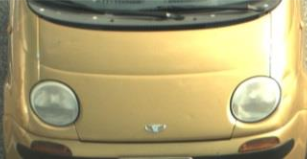
\includegraphics[width=0.3\linewidth]{image/lit/homo1.png}
 & 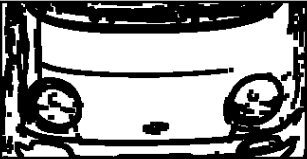
\includegraphics[width=0.3\linewidth]{image/lit/homo3.png} \\
  (a) ROI Image
 & (b) Inverse of Edge Image \\
  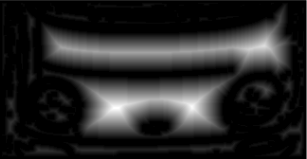
\includegraphics[width=0.3\linewidth]{image/lit/homo2.png} &
  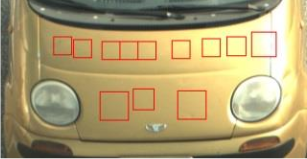
\includegraphics[width=0.3\linewidth]{image/lit/homo4.png} \\
  (c) Distance Transformation &
  (d) Selected Patches\\
 \end{tabular}
 \caption[Homogeneity Patch Search from Input. (a) Region of Interest, (b)
Inverse of Edge Image Using Sobel Operators, (c) Distance Transformation
Calculated using Felzen-szwlb algorithm, (d) Selected Patches Based on Obtained
Distance.]{Homogeneity Patch Search from Input. (a) Region of Interest, (b)
Inverse of Edge Image Using Sobel Operators, (c) Distance Transformation
Calculated using Felzenszawlb algorithm, (d) Selected Patches Based on Obtained
Distance. Image reproduced from \citeA{jeong2017homogeneity}
 \label{fig:colorpatches}}
\end{figure}

As colour histogram is one of the most common mid-level feature used for colour
classification task, \citeA{kim2008deciding} aimed to understand the impact of the number of colour histogram bins used and how different configurations
would affect the performance of matching the histogram bins to colour terms
using distance measures. \citeA{zhang2017vehicle} concluded that the use of histogram bins can effectively reduces the processing time needed while promoting reliable recognition accuracy. The Hue-Saturation-Intensity (HSI) colour space was used in their experiments, with a total of 17 different configurations of combining histogram bins from the three channels (\emph{i.e.} 16 bins for Hue (H), 4 bins for Saturation (S) and 4 bins for Intensity (I)). The results from the experiment shows an average score of 84\%; the best
configuration of (H:8, S:4, I:4) achieving an accuracy of 87.83\% over seven colour classes with 100 images per class.

\citeA{zhang2017vehicle} and \citeA{hu2015vehicle} approached the task of extracting colour categories by implementing a convolutional neural network (CNN) to extract deep features which are then fed into a linear SVM for the classification task. \citeA{zhang2017vehicle} mentioned that state-of-the-art methods typically take the whole image for colour recognition, however many parts of the images such as car windows, wheels, and background contribute negatively to the recognition accuracy. A noise reduction method via saliency detection was proposed in order to boost the performance. While this method achieved a good accuracy of 94\%, the proposed pipeline with saliency detection, deep feature extraction, dual-orientational dimensionality reduction and classifier training incur a high computational cost and is not suitable for real-time applications.

\begin{figure}[!htb] \centering
 %\resizebox{\textwidth}{!}{
\begin{tabular}{cc}
 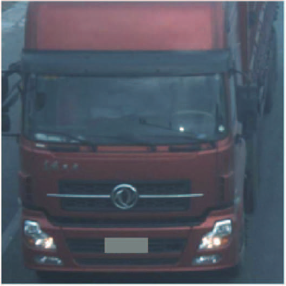
\includegraphics[width=0.4\linewidth]{image/lit/hu1.png} &
 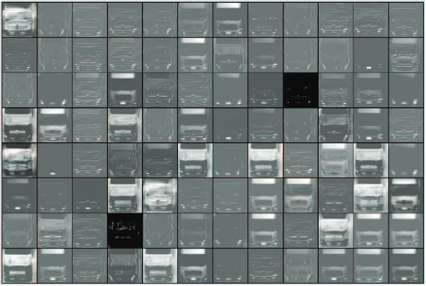
\includegraphics[width=0.6\linewidth]{image/lit/hu2.png} \\
 (a) Input Image & (b) Response Map of the First Convolutional Layer \\
\end{tabular}
%}
\caption[(a) Sample input image and (b) the response from first convolutional layer]{Visualization of first convolutional layer response maps from the deep feature learning method of \citeA{hu2015vehicle}. Images reproduced from
\citeA{hu2015vehicle}.
\label{fig:responseFCL}}
\end{figure}

According to \citeA{hu2015vehicle}, there are two reasons for choosing a SVM classifier over fully-connected (FC) layers (with a softmax classifier) of deep neural network methods. The first reason is the ability of SVMs to perform
better due to regularisation constraints that help overcome over-fitting training data. Regularisation techniques such as dropout can be implemented on FC layers, but its weights will be randomly discarded in an unprincipled manner. Another reason why SVM was chosen as classifier was due to the fact that SVMs have lesser parameters, which makes them less prone to over-fitting. 
% [comment] "easier" may not be the right thing to say
%this makes the fine tuning process easier.
Figure
\ref{fig:responseFCL} illustrates the input image and the response produced by
the first convolutional layer produced in the work of \citeA{hu2015vehicle}. The authors claimed that features derived from the proposed method have advantages over that of hand-crafted methods that perform manual segmentation of sub-regions. This is because the response map from the first convolutional layer contains meaningful ROIs which are effective at distinguishing vehicle colours. Their work achieved an average precision of 93\% with input data of $1920 \times 1080$ pixels resolution. On a whole, while both hand-crafted features and machine-learned features were able to yield accuracies of over 84\%, their proposed solution seemed to have worked well on high resolution data.

\begin{figure}[hbt!]
 \centering
 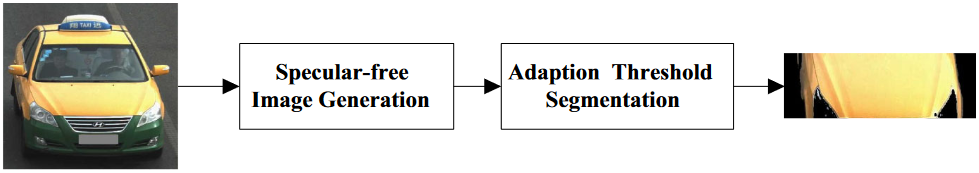
\includegraphics[width=1\textwidth]{image/lit/salient1.png}
 \caption[Vehicle-Colour Saliency Detection]{Vehicle-Colour Saliency Detection.
Reproduced from \citeA{zhang2017vehicle}.}
 \label{fig:Colorsaliency}
\end{figure}

In other related research areas such as vehicle re-identification, several works -- \cite{liu2016deep}, \cite{liu2016deep2} and \cite{shen2017learning}), made use of extracted colour features to assist in the re-identification process. \citeA{liu2016deep} adopted the Probabilistic Latent Semantic Analysis (PLSA) introduced by \citeA{van2009learning}, to extract the colour features (to be discussed in Section~\ref{sec:color2colorterm}). A PLSA model is used to learn the relation between words (colour terms) and images by providing a conditional probability score. Similar to \cite{kim2008deciding}, the images in this work were segmented and represented using L*a*b colour histogram of $10 \times 20 \times 20$ grids. \citeA{liu2016deep2} applied deep learning techniques inspired by a triplet loss network proposed by \citeA{ding2015deep}. The employed network utilised a new loss function to accelerate the training convergence. Eventually, the colour features were extracted using the proposed network. In quite similar fashion, \citeA{shen2017learning} applied a deep learning network to extract the colour features using a Siamese Network with a shared ResNet-50 configuration. The visual features, including colours, were obtained using the features from the global pooling layers.

\vspace{1em}
\subsubsection{Colour to Colour Term Mapping}
\label{sec:color2colorterm}

Colour terms or names, are very useful in real-world applications as compared to colour tuples. According to \cite{van2009learning}, colour names are typically required for image retrieval and image annotation applications due to its affinity to human-level language. Several authors has looked into mapping colour tuples to their respective colour terms. \citeA{van2009learning} proposed several variants of the PLSA model to learn colour names from data obtained Google Images. This was done in order to avoid hand-labelling real-world images with colour names, Figure \ref{fig:van20091} illustrates the types of images retrieved using Google Images. The authors approached this challenge by comparing their methods against 3 chip-based methods. In their work, chip-based methods were described as a colour naming procedure that is performed in a controlled environment where the labels of colour chips are placed on a neutral background under a white light source. Similar to the work of \citeA{van2009learning}, \citeA{yu2018beyond} applied PLSA inversely to estimate the probability of colour values when given a colour term.

\begin{figure}[hbt!]
 \centering
 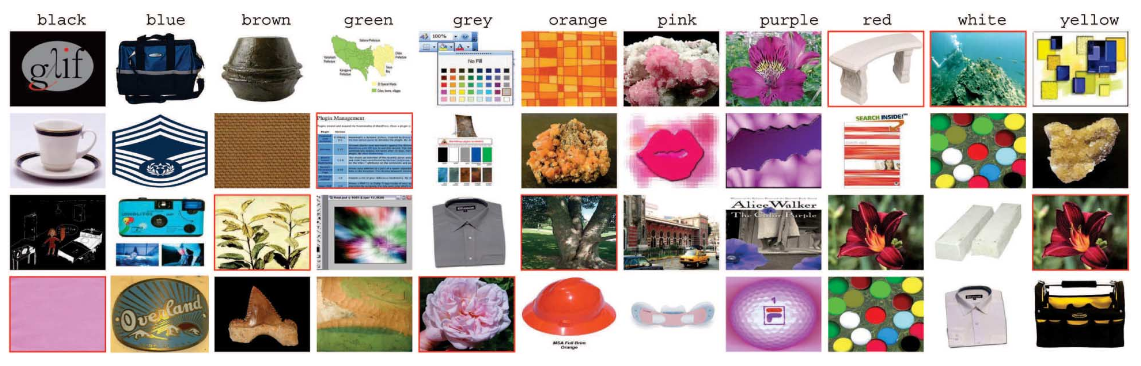
\includegraphics[width=1\textwidth]{image/lit/van20091.PNG}
 \caption[Google-retrieved examples for colour names. The red bounding boxes
 indicate false positives. An image can be retrieved with various colour names,
 such as the flower image which appears in the red and the yellow
 set]{Google-retrieved examples for colour names. The red bounding boxes
 indicate false positives. An image can be retrieved with various colour names,
 such as the flower image which appears in both red and yellow colour sets.
 Reproduced from \citeA{van2009learning}.}
 \label{fig:van20091}
\end{figure}

The PLSA model (as the one proposed in~\cite{van2009learning}) allows multiple colour terms to be named for each image. The pixels in the image (document) is discretised into a finite vocabulary set of $10 \times 20 \times 20$ cubes of L*a*b colour space. Then, the image is represented using a histogram which indicates the number of pixels assigned to each bin (word). Now, given a set of documents $D = \{d_1, d_2, \ldots, d_N\}$ each described in a vocabulary $W = \{w_1, w_2, \ldots, w_M\}$, the words are taken to be generated by latent topics $Z = \{z_1, z_2, \ldots, z_K\}$. In the PLSA model, the conditional probability of a word $w$ in a document $d$ is given by: 
\begin{align} 
    p(w|d) = \sum_{z\in Z}{p(w|z)p(z|d)}
\end{align} 
The aim of $p(w|d)$ is to find latent topics that best explains the observed data, and in this case, finding the colour terms that best describes an image. In their approach, the authors claimed that their proposed method is flexible when new colour terms are introduced to any given system as the model can be trained with a small amount of data as compared to traditional methods that rely on chip based studies.

In the works by \citeA{khan2013discriminative} and \citeA{yu2018beyond}, the authors suggested that extending colour representations to more than the eleven known terms could be beneficial. The authors in \cite{yu2018beyond} proposed a dataset of 28 additional colour terms (a total of 39 terms) which was used in their experiments on several tasks such as visual tracking, person re-identification as well as image classification. One of their experiments shows improvement in classification accuracy by 4\% when increasing from 11 to 25 colour terms.

\begin{figure}[hbt!]
 \centering
 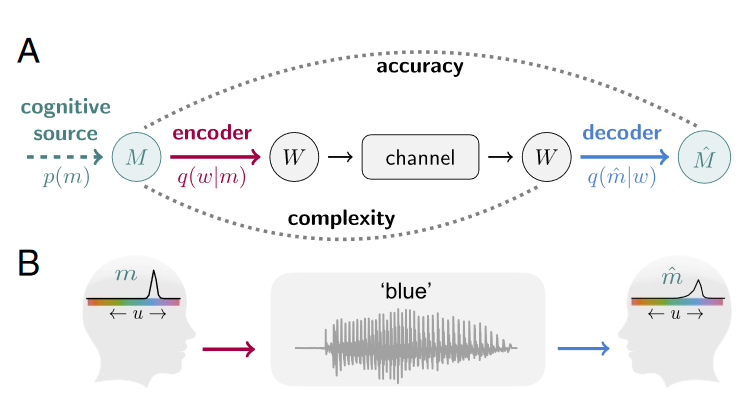
\includegraphics[width=1\textwidth]{image/lit/datacompress1.PNG}
 \caption[(A) Shannon's communication model. In this model, the source
 message $M$ and its reconstruction $\hat{M}$ are distributions over objects
 in the universe $U$. We refer to these messages as meanings. $M$ is compressed
 into a code, or word, W. We assume that $W$ is transmitted over an
 idealised noiseless channel and that the reconstruction $\hat{M}$
 of the source message is based on $W$.
 The accuracy of communication is determined by comparing $M$ and $\hat{M}$,
 and the complexity of the lexicon is determined by the mapping from $M$ to
 $W$. (B) Colour Communication Example, where $U$ is a set of colours, shown
 for simplicity along a single dimension. A specific meaning $m$ is drawn from
 $p(m)$. The speaker communicates $m$ by uttering the word “blue”, and the
 listener interprets blue as meaning $\hat{m}$] {(A)
 \citeA{shannon1948mathematical}'s communication model. In this model, the
 source message $M$ and its reconstruction $\hat{M}$ are distributions over
 objects in the universe $U$. We refer to these messages as meanings. $M$ is
 compressed into a code, or word, W. We assume that $W$ is transmitted over an
 idealised noiseless channel and that the reconstruction $\hat{M}$ of the
 source message is based on $W$. The accuracy of communication is determined by
 comparing $M$ and $\hat{M}$, and the complexity of the lexicon is determined
 by the mapping from $M$ to $W$. (B) Colour Communication Example, where $U$
 is a set of colours, shown for simplicity along a single dimension. A specific
 meaning $m$ is drawn from $p(m)$. The speaker communicates $m$ by uttering the
 word 'blue”, and the listener interprets blue as meaning $\hat{m}$.
 Reproduced from \citeA{zaslavsky2018efficient}.}
 \label{fig:datacompression1}
\end{figure}

Meanwhile, the work of \cite{zaslavsky2018efficient} took on another approach towards
colour tuples mapping. The authors aimed to study efficient compression in colour naming and its evolution. They suggested that colour categories cannot be hard-partitioned in the colour space, whereby instead, a soft-partition approach should be taken. However, the drawback is that with a soft-partition approach, there are transition regions in the colour space that are often inconsistently named. In their work, they approached the challenge of understanding how colours are named from the perspective of data compression. Figure~\ref{fig:datacompression1} illustrates the idea in~\cite{zaslavsky2018efficient}. Succinctly, the goal of this work is to design a Information Bottleneck (IB) compression model that can effectively represent colours terms in different languages.


\begin{comment}
 https://ieeexplore.ieee.org/stamp/stamp.jsp?tp=&arnumber=4982667&tag=1
 https://www.pnas.org/content/pnas/115/31/7937.full.pdf
 https://link.springer.com/content/pdf/10.1007%2Fs00138-017-0902-y.pdf
 https://www.imbs.uci.edu/~kjameson/HinksCardenasKuehniEtAlJOSA2007.pdf
 http://imbs.uci.edu/~kjameson/ECST/Kay_Cook_WorldColorSurvey.pdf
 http://www.munsellcolourscienceforpainters.com/ConversionsBetweenMunsellAndsRGBsystems.pdf
\end{comment}

\vspace{1em}
\subsubsection{Vehicle Motion Extraction \& Representation}
\label{subsec:vehiclemotionextraction}

Vehicle motion is another important feature that can be used to describe activities in a car park surveillance scene. While there are indeed not much research done within the scope and setting of car park surveillance, there has been many works in the general ITS domain which require extraction and analysis of vehicle motions. In most cases where the research setup involves a static camera sensor, the extraction of motions in scene can be broadly divided into two categories:
i) Background subtraction (BGS) methods combined with vehicle centroid position for motion estimation; and ii) Extraction of features (\emph{e.g.} handcrafted descriptors such as Scale-Invariant Feature Transform (SIFT), Histogram of Oriented Gradients (HOG), Haar-like, Kanade-Lucas-Tomasi (KLT), or deeply learned features from convolutional neural networks (CNN)), which can be integrated with optical flow for motion estimation. 
Since the scope of this thesis (Section \ref{subsec:scope}) assumes the vehicles have been detected and localized, hence, only a brief overview of the vehicle motion extraction process will be explored while trajectory representation methods are afforded a more detailed discussion.

BGS methods are often used as there is no necessity for prior training on a machine to recognise vehicles. Instead, this method relies entirely on the captured motions and the scene. Several
authors (\citeA{wang2016research, luvizon2017video, apeltauer2015automatic})
extracted vehicle motion information via BGS method. Generally, a clean model of
background information is first obtained. When a new object is introduced on the
scene in the current frame, the differences between the background information and the current frame is extracted to indicate changes in the scene. When the objects (also known as blobs) are moving in the scene, the regions obtained from the subtraction
process would correspond to motion information. Figure \ref{fig:bgs2}
illustrates the process of extracting vehicle motion using BGS. BGS methods are typically very sensitive to noise, outliers and illumination changes. So, in order to further increase the accuracy of extracting vehicle motion, these works filter out blobs that do not match the desired object dimensions.

\begin{figure}[hbt!]
  \centering
 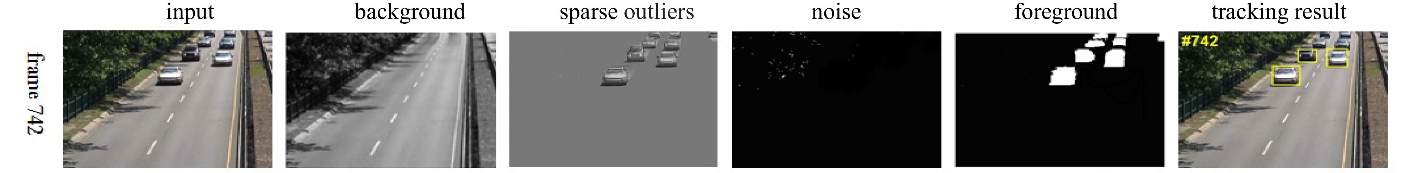
\includegraphics[width=1\textwidth]{image/lit/bgs.PNG}
  \caption[Vehicle Motion Extraction using Background Subtraction. From left:
  Input, Background Model, Sparse Outlier, Noise, Foreground, Tracking Result]
  {Vehicle Motion Extraction using Background Subtraction. %From left: Input, Background Model, Sparse Outlier, Noise, Foreground, Tracking Result.
  Reproduced from \citeA{yang2017real}.}
\label{fig:bgs2}
\end{figure}

Contrary to BGS methods, feature extraction methods rely on the visual information of vehicles such as colours, texture and shapes. In the case of vehicles, the combination of different components such as the windscreen, the chassis, wheels, doors and windows does add up to constitute a vehicle. These visual information are learned to model and identify vehicles. In an attempt to count vehicles from 500 hours of
videos, \citeA{lessard2016countingapp} applied the methods of~\citeA{saunier2006feature} to extract motion information using the KLT tracker. These extracted features were grouped into unique trajectories that varies
depending on the targeted scene. In their work, scenes were allocated up to
16 different possible types of trajectories (for the case of a four-legged intersection or `crossroad'). Using this method, the authors was
able to uniquely identify the different types of motion. However, this method limits the types of trajectories captured, and is not feasible when dealing with more complex scenarios such as a large car park as there are too many possible trajectories types to account for. Furthermore, the process of annotating data in this work is too laborious 
% comment: added from the paper
that the authors chose to use the results from a commercial provider of traffic counts (guaranteed 95\% accuracy rate) as the ground-truth with additional random checks made to ensure reliability.

Instead of manually allocating unique trajectories, \citeA{momin2015vehicle}
took a different approach towards categorising motions. The authors combined
Haar-like features along with BGS methods to extract motion information. The
extracted vehicle motions at each point in time is then split into one of the
four directions (LEFT, RIGHT, UP, DOWN). Similarly, the work of
\citeA{feris2012large} splits the motion of vehicles into 12 motion directions
depending on the orientation of the vehicles. These motion directions were
assigned for every $\ang{30}$ (\emph{e.g.}: $\ang{0}-\ang{30}, \ang{30}-\ang{60}, \ldots,
\ang{330}-\ang{360}$). A motion direction histogram is built such that the bin
which receives the highest number of votes are assigned as the main motion direction. Likewise, \citeA{castanon2016retrieval} categorised motions into 9 histogram of motion bins using the aggregate motion which was computed using pixel-level optical flow (Horn and Schunck method). These 9 bins correspond to the eight cardinal directions along with one idle bin to denote the absence of significant motion.

With the goal of designing huge repositories of moving vehicle trajectories, \citeA{d2015designing} represent trajectories using spatio temporal cubes (See
Figure~\ref{fig:spatiocube}). Similarly, \citeA{lai2015video} represented human trajectories in the same manner. In addition to that, the authors used B-spline curve fitting methods to further reduce noisy information. Since different degrees of curve fitting lead to different results (see Figure~\ref{fig:spatiocube2}), the authors proposed to merge multiple curves of different degrees to strike a balance between noise removal and accuracy. These works demonstrated that this method of trajectory representation using spatio temporal cubes is intuitive as it is able to capture and relay information accurately. However, the downside of this method is that the accuracy of data representation heavily relies on the
number of spatio-temporal cubes used.

\begin{figure}[hbt!]
  \centering
  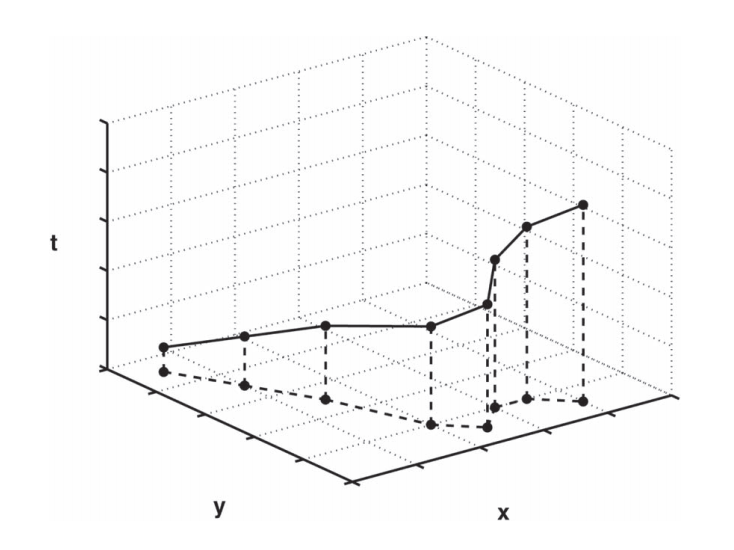
\includegraphics[width=.5\textwidth]{image/lit/spatiotemporal.PNG}
  \caption[Representation of Trajectories in a Spatio-temporal Cube]
 {Representation of Trajectories in a Spatio-temporal Cube. Reproduced from
 \citeA{d2015designing}.}
  \label{fig:spatiocube}
\end{figure}

\begin{figure}[hbt!]
  \centering
  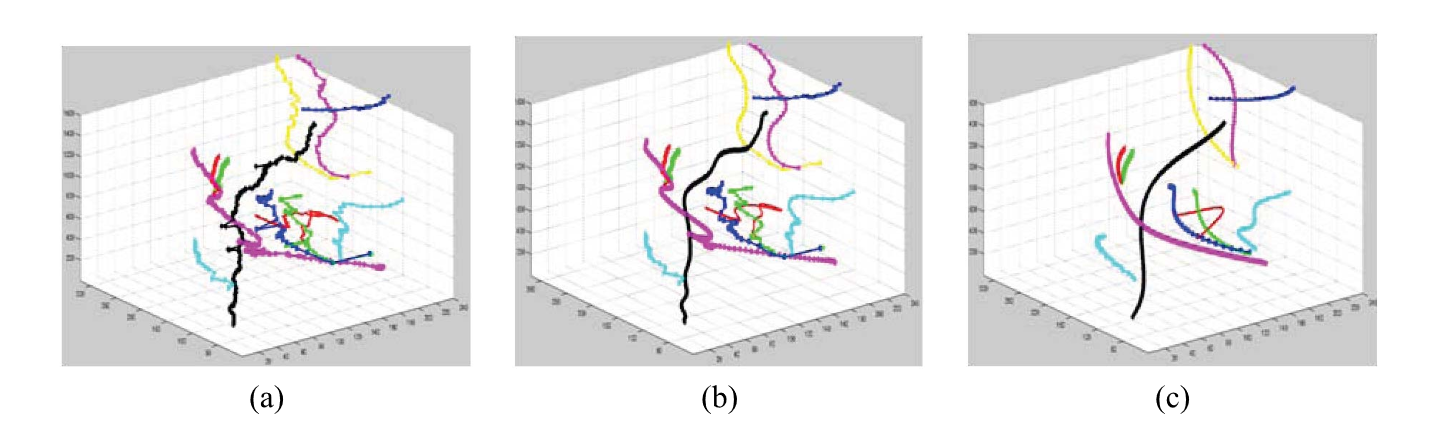
\includegraphics[width=1\textwidth]{image/lit/spatiotemporal2.PNG}
  \caption[Representation of Human Trajectories in a Spatio-temporal Cube. (a)
  Original Object Trajectories; (b) Curve fitting results using high degrees;
  (c) Curve fitting results using low degrees] {Representation of Human
  Trajectories in a Spatio-temporal Cube. (a) Original Object Trajectories; (b)
  Curve fitting results using high degrees; (c) Curve fitting results using low
  degrees. Reproduced from \citeA{lai2015video}.}
  \label{fig:spatiocube2}
\end{figure}



\vspace{1em}
\subsection{Object Semantics Retrieval}

According to the survey by \cite{chandran2017review}, object retrieval
algorithms can be broadly divided into two categories: i) String Matching
Algorithm, and ii) Sketch Matching Algorithm. String matching algorithms
typically converts subjects into a set of known keywords and match them using
its semantic meanings. However, \citeA{bhaumik2016hybrid} suggests that
Content-based Video Retrieval (CVBR) can be classified into three categories: i)
Classical Approach, ii) Soft Computing and iii) Hybrid Soft Computing. Figure
\ref{fig:cvbr} shows the classification of various approaches used in CVBR
systems.

\begin{figure}[hbt!]
  \centering
  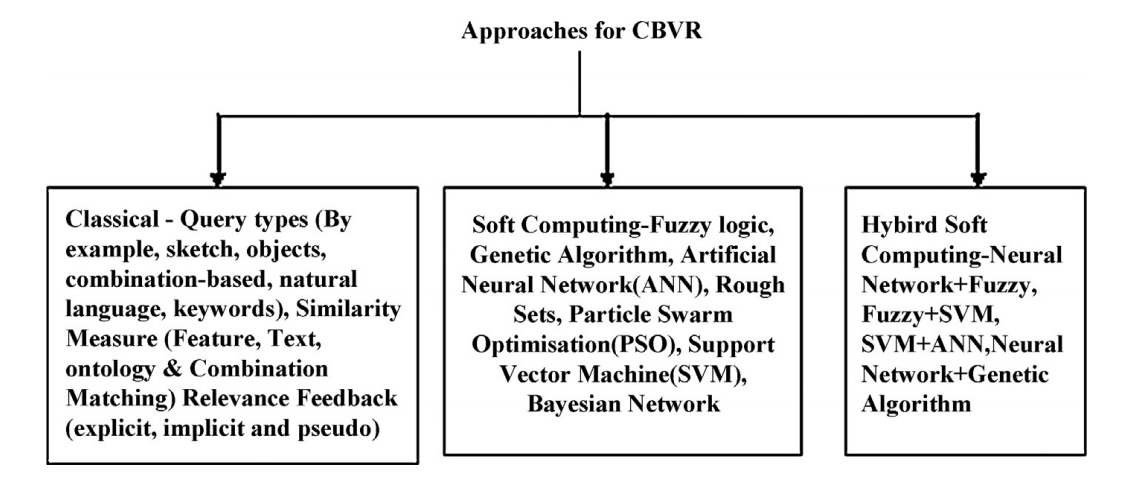
\includegraphics[width=.9\textwidth]{image/lit/cvbr.PNG}
  \caption[Classification of Approaches Used in Content-based Video Retrieval
  Systems] {Classification of Approaches Used in Content-based Video Retrieval
  Systems. Reproduced from \citeA{bhaumik2016hybrid}.}
  \label{fig:cvbr}
\end{figure}

Several authors~\cite{feris2012large,momin2015vehicle,yang2015semantic} implemented string matching algorithms, a classical approach, into their work. In the case of vehicle trajectories, often the queries are represented in the form of keywords/phrases such as "Turning into junction A" or "Enter from entrance B". The approach suggested by these authors attempt to simulate natural language queries that would be provided by end users. However, when dealing with large datasets that contain a variety of scenes, it is both tedious and difficult to establish consistency when manually assigning keywords. In the review by~\citeA{bhaumik2016hybrid}, it was suggested that the use of textual
queries has been proven to be ineffective in video retrieval systems. This is
because keywords may not be able to intuitively capture the full range of semantic content
required by a end user.

Within the scope of exemplar-based retrieval, the use of sketches is
another classical method applied by retrieval engines. The classic work of~\citeA{flickner1995qbic} proposed a retrieval engine which takes in queries in the form of features such as object motion, colours, shapes and texture. Similarly,
\citeA{Cheng_2013_ICCV} also took on the challenge of retrieving contents based
on the detected salient regions. However, the author only focused on the retrieval of still images instead of videos. In terms of retrieval of trajectories,~\citeA{lai2015video} allowed end users to draw trajectories that
matches the desired results. These drawn trajectories are then fitted using
B-spline curves which will then be use to match against trajectory records stored in
the database. The authors reported an average accuracy of 73.28\% when tested
against 5 video sequence with an average length of 1,500 frames. Figure
\ref{fig:drawquery1} illustrates the hand drawn trajectories which are converted
into query inputs.


\begin{figure}[hbt!]
  \centering
  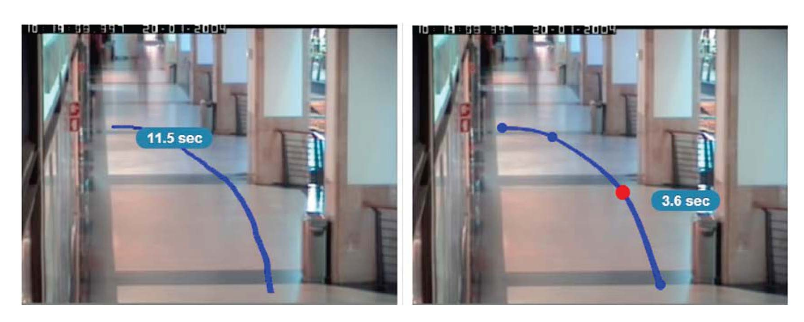
\includegraphics[width=.9\textwidth]{image/lit/trajdraw1.PNG}
  \caption[\textit{Left}: Hand-drawn Trajectory for Retrieval Purposes.
  \textit{Right}: Resulting Simplified B-spline Curve for Easier Manipulation of
  Trajectory] {\textit{Left}: Hand-drawn Trajectory for Retrieval Purposes.
  \textit{Right}: Resulting Simplified B-spline Curve for Easier Manipulation of
  Trajectory. Reproduced from \citeA{lai2015video}.}
  \label{fig:drawquery1}
\end{figure}

Similar to the approach taken by \cite{lai2015video}, in an airborne video
setting, \citeA{castanon2016retrieval} also allowed end users to draw the
trajectories which are then segmented and used for retrieval purposes. The
authors applied dynamic programming techniques to search for the best match.
Along with that, the authors also reported that their approach takes an average
of 2.9 seconds to process simpler trajectories while taking up to 4.32 seconds to process complicated ones. The processing speed was averaged out across 2000
frames against stored data that was 13.8 minutes in length. Their approach appears to be rather computationally expensive. However, the authors reported significantly
better results when compared to other methods. Figure~\ref{fig:drawquery2}
illustrates their proposed GUI and the input queries.
%while Figure~\ref{fig:rocresult} reports the performance of the proposed method.
\begin{figure}[hbt!]
  \centering
  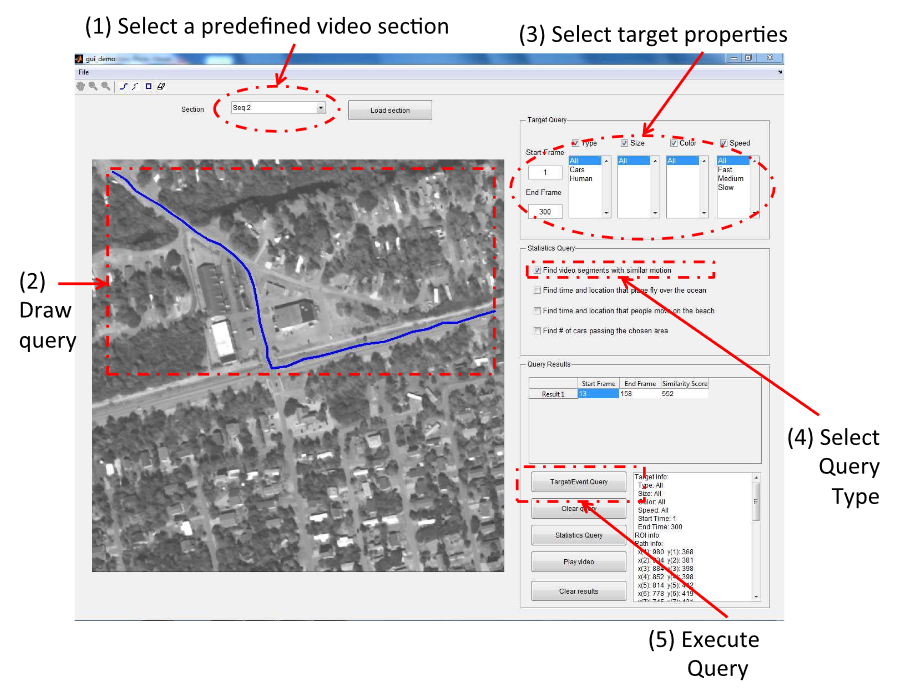
\includegraphics[width=.6\textwidth]{image/lit/trajdraw2.PNG}
  \caption[Graphical User Interface and the Input Trajectory] {Graphical User
  Interface and the Input Trajectory. Reproduced from
  \citeA{castanon2016retrieval}.}
\label{fig:drawquery2}
\end{figure}

\vspace{1em}
\subsection{Summary of Background Study}

This chapter started off with some  fundamental background study on some key concepts such as the quantisation process and distance measures which is repeatedly found in this work. Furthermore, some background on the human visual system and the various colour models and terms were also explored to understand the relation between them. 
Next, literature in the various Intelligent Transportation Systems (ITS) was reviewed. Being a huge domain, there has been a substantial increase of research done on the various sub-domains. This is 
%partly motivated by the bloom of available datasets, but 
primarily motivated by security concerns on how video data can be used for surveillance purposes effectively.

The reviews were presented in various categories to provide a broad perspective on the diverse aspects related to this work. 
\citeA{liu2016deep} mentioned that appearance features such as colours, shapes, and types very effective at filtering out dissimilar vehicles in real-world scenes. 
While true, a majority of the presented literature worked on high resolution data which is atypical toward real-world surveillance footages.
The reviewed literature also shows disparity on how vehicle colours were determined.
Hence, this thesis aims to explore how vehicle colours can be extracted correctly with colour terms that are agreeable with end users while utilising lower resolution data which is more readily found in surveillance data.

In terms of vehicle motion and representation, we notice a gap on how these motions are represented. Majority of these literature describes these motion in the cardinal directions or even in angles. These descriptions lacks intuitive notion without proper context of location, this thesis aims to introduce an intuitive representation of the vehicle motions.
As suggested by \cite{bhaumik2016hybrid}, the use of textual queries has been proven ineffective in video retrieval systems, this work aims to present a retrieval engine using sketch matching algorithms against the intuitive vehicle motion representation. It is also noted that several approach takes an average of 2.9 seconds to process simple trajectory and up to 4.32 seconds for complicated trajectories against 13.8 minutes of video data. This calls for a better approach in retrieving video footages especially over long term surveillance footage.


%\begin{figure}[hbt!]
%  \centering
%  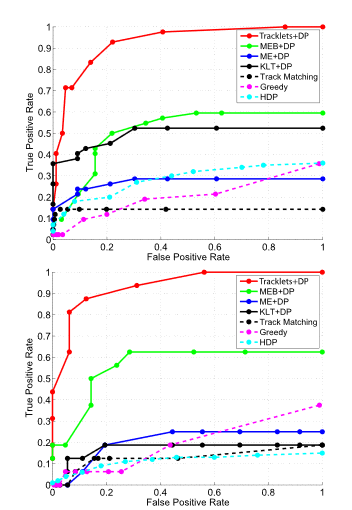
\includegraphics[width=.6\textwidth]{image%/lit/roc.PNG}
%  \caption[ROC Curve for Cars and Human Trajectories in Airborne Data]
%  {ROC Curve for Cars and Human Trajectories in Airborne Data Reproduced
%  from \citeA{castanon2016retrieval}.}
% \label{fig:rocresult}
%\end{figure}
%

